\chapter{Interest Rate Products}

%%%%%%%%%%%%%%%%%%%%%%%%%%%%%%%%%%%%%%%%%%%%%%%%%%%%%%%%%%%%%%%%%%%%%%%%%%%%%%
\section{Day count conventions}

We give the formula for calculating year fraction between two days $d_1$ and
$d_2$ given two reference dates $d_3$ and $d_4$, using the Actual/Actual ICMA
convention.

\begin{equation}
  YF(d_1,d_2) = \frac{Days(d_1,d_2)}{f \times Days(d_3, d_4)},
\end{equation}
here $f$ is the payment frequency. If $f$ is not specified, it can be estimated
by
\begin{equation}
  f = \frac{12.0}{Integer(0.5 + 12 * (d_2 - d_1) / 365.0)}.
\end{equation}

If reference dates $d_3$ and $d_4$ are not given, we can usually set $d_3=d_1$
and $d_4=d_2$, and the year fraction formula becomes
\begin{equation}
  YF(d_1,d_2) = \frac{Days(d_1,d_2)}{f \times Days(d_1, d_2)}
              = \frac{1}{f}.
\end{equation}





%%%%%%%%%%%%%%%%%%%%%%%%%%%%%%%%%%%%%%%%%%%%%%%%%%%%%%%%%%%%%%%%%%%%%%%%%%%%%%
\section{Prototypical Coupon Bond}
A prototypical coupon bond is a contract that pays at dates 
$\{T_1,T_2,\cdots,T_{n}\}$ the amounts of $\{c_1,c_2,\cdots,c_n\}$. Typically
the cashflows are defined as $c_i=N\delta_i K$ for $i<n$, and 
$c_n=N\delta_n K+N$ where $K$ is a fixed coupon rate, $N$ is the face value,
and $\delta_j$ be the year fraction between dates $T_{j-1}$ and $T_{j}$,

%%%%%%%%%%%%%%%%%%%%%%%%%%%%%%%%%%%%%%%
\begin{figure}
  \begin{tikzpicture}[scale=0.9]
    \draw (-3.5,0) -- (2.8,0);
    \drawbreakright{2.8}{0}
    \drawbreakleft{4.2}{0}
    \draw (4.2,0) -- (9.3,0);
    \draw (-2,0) node[below] {$T_0$} -- (-2,0.2);

    \draw [->, >=triangle 90] 
      (0,0) node[below] {$T_1$} -- (0,2) node[above] {$c_1$} ;
    \draw [->, >=triangle 90] 
      (2,0) node[below] {$T_2$} -- (2,2) node[above] {$c_2$} ;
    \draw [->, >=triangle 90] 
      (5,0) node[below] {$T_{n-1}$} -- (5,2) node[above] {$c_{n-1}$} ;
    \draw [->, >=triangle 90] 
      (7,0) node[below] {$T_{n}$} -- (7,3) node[above] {$c_{n}$} ;
  \end{tikzpicture} 
  \caption{A prototypical coupon bond pays at dates
           $\{T_1,T_2,\cdots,T_{n}\}$ the fixed amounts of 
           $\{c_1,c_2,\cdots,c_n\}$.}
\end{figure}
%%%%%%%%%%%%%%%%%%%%%%%%%%%%%%%%%%%%%%%

The current value of the coupon bond is
\begin{equation}
  CB(t,\{T_j\}_{j\le n},\{c_j\}_{j\le n}) = \sum_{i=1}^n c_i D_{tT_i}.
\end{equation}

%%%%%%%%%%%%%%%%%%%%%%%%%%%%%%%%%%%%%%%%%%%%%%%%%%%%%%%%%%%%%%%%%%%%%%%%%%%%%%
\section{Prototypical floating-rate note}
A prototypical floating-rate note pays at dates
$\{T_1,T_2,\cdots,T_{n}\}$ the LIBOR rates that reset at previous dates
$\{T_0,T_1,\cdots,T_{n-1}\}$, plus the notional on $T_n$. 

%%%%%%%%%%%%%%%%%%%%%%%%%%%%%%%%%%%%%%%
\begin{figure}
  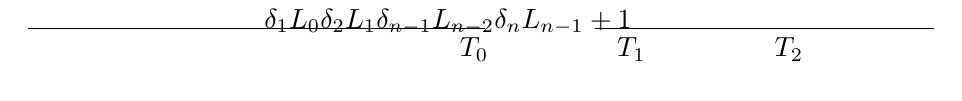
\begin{tikzpicture}[scale=1]
    \draw (-3,0) -- (2.8,0);
    \drawbreakright{2.8}{0}
    \drawbreakleft{4.2}{0}
    \draw (4.2,0) -- (8.5,0);

    % floating payments using snake lines (with my own code for \drawsnake)
    \drawsnake{(0,0)}{(0,1.1)}{$\delta_{1} L_0$}
    \drawsnake{(2,0)}{(2,1.6)}{$\delta_{2} L_1$}
    \drawsnake{(5,0)}{(5,1.1)}{$\delta_{n-1} L_{n-2}$}
    \drawsnake{(7,0)}{(7,1.6)}{$\delta_{n} L_{n-1} + 1$}

    \draw (-2,0) node[below]{$T_0$} ; % text only
    \draw (0,0) node[below]{$T_1$} ; % text only
    \draw (2,0) node[below]{$T_2$} ; % text only
    \draw (5,0) node[below]{$T_{n-1}$} ; % text only
    \draw (7,0) node[below]{$T_{n}$} ; % text only

  \end{tikzpicture} 
  \caption{A prototypical floating rate note pays on dates 
           $\{T_1,T_2,\cdots,T_{n}\}$ the LIBOR rates that reset at previous 
           dates $\{T_0,T_1,\cdots,T_{n-1}\}$. Here we use
           abbreviation $L_j$ for $L_j[T_j,T_{j+1}]$ and the notional is 1. }
\end{figure}
%%%%%%%%%%%%%%%%%%%%%%%%%%%%%%%%%%%%%%%

The current value of the note is
\begin{equation}
  FRN(t,\{T_j\}_{j\le n}) = D_{tT0}.
\end{equation}


%%%%%%%%%%%%%%%%%%%%%%%%%%%%%%%%%%%%%%%%%%%%%%%%%%%%%%%%%%%%%%%%%%%%%%%%%%%%%%
\section{Interest Rate Swaps}
An interest rate swap is an agreement between two counterparties
to exchange a series of cashflows on pre-agreed dates in the future (see Figure
\ref{F:swap}). In general the payment frequencies of the fixed and floating legs
are different. A payer's swap pays fixed rate $K$ and receives the floating rate, 
while a receiver's swap pays floating rate and receives fixed rate.

Let $\{T_0,T_1,\cdots,T_{n-1}\}$ be the reset dates, and
$\{T_1,T_2,\cdots,T_{n}\}$ be the payment dates of the floating leg, and
$\{S_0,S_1,\cdots,S_{m-1}\}$ be the reset dates, and
$\{S_1,S_2,\cdots,S_{n}\}$ be the payment dates of the fixed leg. 
Let $\delta^S_j$ be the year fraction between dates $S_{j-1}$ and $S_{j}$,
and let $\delta^T_{j}$ be the year fraction between dates $T_{j-1}$ and 
$T_{j}$. For a payer's swap, the payoff at time $T_j$ is
\[
  \delta^T_j L_{T_{j-1}}[T_{j-1},T_j]  \qquad j=1,2,\cdots,n
\]
and at the time $S_j$, the payoff is
\[
  - \delta^S_j K  \qquad j=1,2,\cdots,m.
\]

%%%%%%%%%%%%%%%%%%%%%%%%%%%%%%%%%%%%%%%
\begin{figure}
  \begin{tikzpicture}[scale=1]
    \draw (-3,0) -- (2.8,0);
    \drawbreakright{2.8}{0}
    \drawbreakleft{4.2}{0}
    \draw (4.2,0) -- (8.5,0);

    % floating payments using snake lines (with my own code for \drawsnake)
    \drawsnake{(0,0)}{(0,1.1)}{$\delta^T_{1} L_0$}
    \drawsnake{(2,0)}{(2,1.6)}{$\delta^T_{2} L_1$}
    \drawsnake{(5,0)}{(5,1.1)}{$\delta^T_{n-1} L_{n-2}$}
    \drawsnake{(7,0)}{(7,1.6)}{$\delta^T_{n} L_{n-1}$}

    \draw (-2,0) node[below right]{$S_0$} node[above right]{$T_0$} ; % text
    \draw (-2,-0.2) -- (-2,0.2);
    \draw (0,0) node[above right] {$T_1$} -- (0,0.2);
    \draw (5,0) node[above right] {$T_{n-1}$} -- (5,0.2);

    \draw [->, >=triangle 90] 
      (2,0) node[above right]{$T_2$} node[below right] {$S_1$} 
      -- (2,-1) node[below] {$\delta^S_{1}K$} ;
    \draw [->, >=triangle 90] 
      (7,0) node[above right]{$T_{n}$} node[below right] {$S_{m}$} 
      -- (7,-1) node[below] {$\delta^S_{m}K$} ;
  \end{tikzpicture} 
  \caption{A payer's swap pays fixed and receives floating rate. Here we use
           abbreviation $L_j$ for $L_j[T_j,T_{j+1}]$. In this example the
           floating leg pays twice as frequent as the fixed leg, i.e. $n=2m$.}
  \label{F:swap}
\end{figure}
%%%%%%%%%%%%%%%%%%%%%%%%%%%%%%%%%%%%%%%

The price of the fixed leg at time $t<T_0$ is
\[
  K \sum_{j=1}^m \delta^S_j D_{tS_j},
\]
while the price of the floating leg is simply
\[
  \sum_{j=1}^n \delta^T_j L_{T_{j-1}}[T_{j-1},T_j] D_{tT_j}
    = D_{tT_0} - D_{tT_n}.
\]
And the price of a payer's swap is the difference between the floating leg and
the fixed leg:
\begin{equation}
  PFS(t,\{T_j\}_{j\le n},\{S_j\}_{j\le m},K)
    = D_{tT_0} - D_{tT_n} - K\sum_{j=1}^m \delta^S_j D_{tS_j}.
\end{equation}
Similarly the price of a receiver's swap equals the fixed leg substracts the
floating leg:
\begin{equation}
  RFS(t,\{T_j\}_{j\le n},\{S_j\}_{j\le m},K)
    = -D_{tT_0} + D_{tT_n} + K\sum_{j=1}^m \delta^S_j D_{tS_j}.
\end{equation}


The par swap rate is the fixed rate of the swap such that the swap is at the 
money, i.e.
\begin{equation} \label{E:swap}
  y_n(t) \equiv y(t,\{T_j\}_{j\le n},\{S_j\}_{j\le m}) 
    = \frac{ D_{tT_0} - D_{tT_n} }{ \sum_{j=1}^m \delta^S_j D_{tS_j} },
\end{equation}


%%%%%%%%%%%%%%%%%%%%%%%%%%%%%%%%%%%%%%%%%%%%%%%%%%%%%%%%%%%%%%%%%%%%%%%%%%%%%%
\section{Caps and Floors}
An interest rate cap is made up of a series of caplets. 
\marginnote{Cap}
Let $\{T_0,T_1,\cdots,T_{n-1}\}$ be the reset dates, and
$\{T_1,T_2,\cdots,T_{n}\}$ be the payment dates of the cap, 
and let $\delta_{j}$ be the year fraction between dates $T_{j-1}$ and $T_j$.
At time $T_j,j=1,2,\cdots n$, the payoff is
\begin{equation} \label{E:cap}
  \delta_j \left( L_{T_{j-1}}[T_{j-1},T_j] - K \right)_+,
\end{equation}
where $K$ is the strike for the cap (see Figure \ref{F:cap}).

%%%%%%%%%%%%%%%%%%%%%%%%%%%%%%%%%%%%%%%
\begin{figure}
  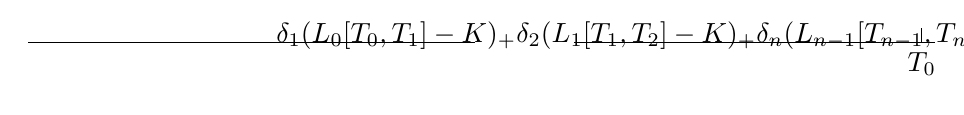
\begin{tikzpicture}[scale=0.9]
    \draw (-3.5,0) -- (2.8,0);
    \drawbreakright{2.8}{0}
    \drawbreakleft{4.2}{0}
    \draw (4.2,0) -- (9.3,0);
    \drawsnake{(0,0)}{(0,2.1)}{$\delta_{1} (L_0[T_0,T_1]-K)_+$}
    \drawsnake{(2,0)}{(2,1.4)}{$\delta_{2} (L_1[T_1,T_2]-K)_+$}
    \drawsnake{(5,0)}{(5,1.5)}{}
    \drawsnake{(7,0)}{(7,2)}{$\delta_{n} (L_{n-1}[T_{n-1},T_{n}]-K)_+$}
    \draw (-2,0) node[below] {$T_0$} -- (-2,0.2);
    \draw (0,0) node[below] {$T_1$} ;
    \draw (2,0) node[below] {$T_2$} ;
    \draw (5,0) node[below] {$T_{n-1}$};
    \draw (7,0) node[below] {$T_{n}$} ;
  \end{tikzpicture} 
  \caption{A cap is made up of a series of caplets.
    The reset dates are $T_0,T_1,\cdots,T_{n-1}$, the payment dates are
    $T_1,T_2,\cdots,T_{n}$. The payoff at payment dates follows 
    Equation \ref{E:cap}.}
  \label{F:cap}
\end{figure}
%%%%%%%%%%%%%%%%%%%%%%%%%%%%%%%%%%%%%%%

Similarly an interest rate floor is made up of a series of floorets. 
\marginnote{Floor}
Let $\{T_0,T_1,\cdots,T_{n-1}\}$ be the reset dates, and
$\{T_1,T_2,\cdots,T_{n}\}$ be the payment dates of the floor, 
and let $\delta_{j}$ be the year fraction between dates $T_{j-1}$ and $T_j$.
At time $T_j,j=1,2,\cdots n$, the payoff is
\begin{equation} \label{E:cap}
  \delta_j \left( K - L_{T_{j-1}}[T_{j-1},T_j] \right)_+,
\end{equation}
where $K$ is the strike for the floor.


